\chapter{Systemmodelle}

\section{Anwendungsfälle}
    % Anwendungsfall Webinterface
    \subsection{Bedienung des Webinterface}
        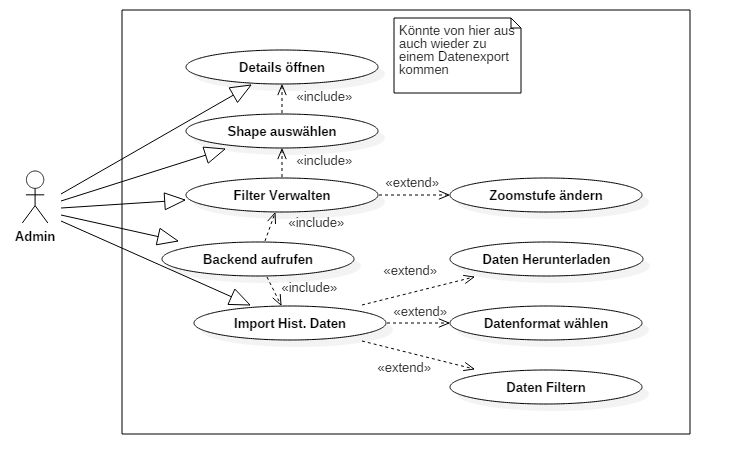
\includegraphics[width=1\linewidth]{diagrams/UseCaseDiagram1.png}
       
       Dieser Anwendungsfall beschreibt die Bedienung des Webinterface. Dem Nutzer stehen folgende Aktionen zur Verfügung:
       \begin{itemize}
            \item Karte anzeigen
            \item Anzeige anpassen
            \item Daten exportieren
            \item Export anpassen
        \end{itemize}
        Nachdem der Nutzer auf das Webinterface zugreift, kann er sich die Karte anzeigen lassen. Diese visualisiert die Daten, welche 
        vom Server durch KafkaStreams bereitgestellt werden. Diese können Echtzeit-, sowie historische Daten enthalten.  Der Server führt 
        im Hintergrund Vorberechnungen zur schnelleren Visualisierung durch. Die Anzeige der Karte, sowie des gesamten Interfaces lässt sich 
        an die Wünsche des Nutzers anpassen, beispielsweise durch die Einbeziehung von Graphen zur besseren Darstellung. Die 
        Datenbestände lassen sich herunterladen und in das gewünschte Format exportieren. Durch Beschränkung der Datenmengen auf 
        bestimmte Zeitintervalle, Datentypen und Wertebereiche kann der Export weiter angepasst werden.
        
    % Anwendungsfall Admin-GUI
    \subsection{Bedienung der Konfigurations-GUI}
        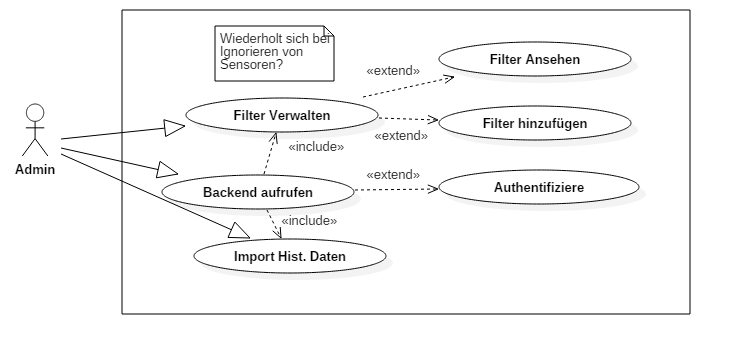
\includegraphics[width=1\linewidth]{diagrams/UseCaseDiagram2.png}
        
        Dieser Anwendungsfall beschreibt die Bedienung der Konfigurations-GUI. Dem Admin stehen folgende Aktionen zur Verfügung:
        \begin{itemize}
            \item Server initialisieren
            \item KafkaStreams verwalten
            \item Datenbestand importieren
            \item Server warten
        \end{itemize}
        Um den Server und damit die Applikation zu starten, greift der Nutzer auf die Konfigurations-GUI zu. Er initialisiert den gestartenen 
        Server, indem ein KafkaStream, bzw. ein Datenbestand eingefügt wird, welcher in einen Stream umgewandelt wird. Dieser wird 
        daraufhin überprüft. Gibt es keine Probleme, so können die Nutzer des Webinterfaces nun die Streams vom Server empfangen. Außerdem ist 
        es nun möglich, die KafkaStreams auf dem Server zu verwalten. Man kann neue Streams hinzufügen, Vorhandene entfernen und 
        enthaltene Sensoren und Sensorendaten anzeigen. Weiterhin lässt sich der Server durch die Konfigurations-GUI warten. Man kann ihn 
        starten, sowie beenden um Analysen durchzuführen und eventuelle Fehler zu beheben.
        
\section{Aktivitätsdiagramm}
    % Aktivitätsdiagramm
    \subsection{}
        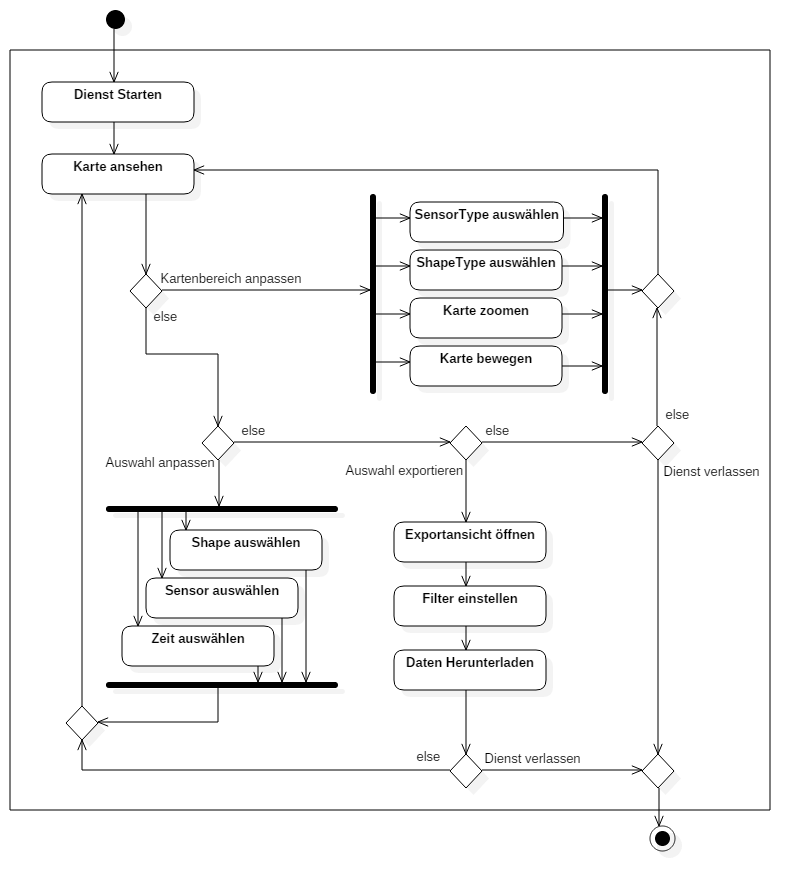
\includegraphics[width=1\linewidth]{diagrams/ActivityDiagram1.png}

        